% Options for packages loaded elsewhere
% Options for packages loaded elsewhere
\PassOptionsToPackage{unicode}{hyperref}
\PassOptionsToPackage{hyphens}{url}
\PassOptionsToPackage{dvipsnames,svgnames,x11names}{xcolor}
%
\documentclass[
  letterpaper,
  DIV=11,
  numbers=noendperiod]{scrartcl}
\usepackage{xcolor}
\usepackage{amsmath,amssymb}
\setcounter{secnumdepth}{-\maxdimen} % remove section numbering
\usepackage{iftex}
\ifPDFTeX
  \usepackage[T1]{fontenc}
  \usepackage[utf8]{inputenc}
  \usepackage{textcomp} % provide euro and other symbols
\else % if luatex or xetex
  \usepackage{unicode-math} % this also loads fontspec
  \defaultfontfeatures{Scale=MatchLowercase}
  \defaultfontfeatures[\rmfamily]{Ligatures=TeX,Scale=1}
\fi
\usepackage{lmodern}
\ifPDFTeX\else
  % xetex/luatex font selection
\fi
% Use upquote if available, for straight quotes in verbatim environments
\IfFileExists{upquote.sty}{\usepackage{upquote}}{}
\IfFileExists{microtype.sty}{% use microtype if available
  \usepackage[]{microtype}
  \UseMicrotypeSet[protrusion]{basicmath} % disable protrusion for tt fonts
}{}
\makeatletter
\@ifundefined{KOMAClassName}{% if non-KOMA class
  \IfFileExists{parskip.sty}{%
    \usepackage{parskip}
  }{% else
    \setlength{\parindent}{0pt}
    \setlength{\parskip}{6pt plus 2pt minus 1pt}}
}{% if KOMA class
  \KOMAoptions{parskip=half}}
\makeatother
% Make \paragraph and \subparagraph free-standing
\makeatletter
\ifx\paragraph\undefined\else
  \let\oldparagraph\paragraph
  \renewcommand{\paragraph}{
    \@ifstar
      \xxxParagraphStar
      \xxxParagraphNoStar
  }
  \newcommand{\xxxParagraphStar}[1]{\oldparagraph*{#1}\mbox{}}
  \newcommand{\xxxParagraphNoStar}[1]{\oldparagraph{#1}\mbox{}}
\fi
\ifx\subparagraph\undefined\else
  \let\oldsubparagraph\subparagraph
  \renewcommand{\subparagraph}{
    \@ifstar
      \xxxSubParagraphStar
      \xxxSubParagraphNoStar
  }
  \newcommand{\xxxSubParagraphStar}[1]{\oldsubparagraph*{#1}\mbox{}}
  \newcommand{\xxxSubParagraphNoStar}[1]{\oldsubparagraph{#1}\mbox{}}
\fi
\makeatother


\usepackage{longtable,booktabs,array}
\newcounter{none} % for unnumbered tables
\usepackage{calc} % for calculating minipage widths
% Correct order of tables after \paragraph or \subparagraph
\usepackage{etoolbox}
\makeatletter
\patchcmd\longtable{\par}{\if@noskipsec\mbox{}\fi\par}{}{}
\makeatother
% Allow footnotes in longtable head/foot
\IfFileExists{footnotehyper.sty}{\usepackage{footnotehyper}}{\usepackage{footnote}}
\makesavenoteenv{longtable}
\usepackage{graphicx}
\makeatletter
\newsavebox\pandoc@box
\newcommand*\pandocbounded[1]{% scales image to fit in text height/width
  \sbox\pandoc@box{#1}%
  \Gscale@div\@tempa{\textheight}{\dimexpr\ht\pandoc@box+\dp\pandoc@box\relax}%
  \Gscale@div\@tempb{\linewidth}{\wd\pandoc@box}%
  \ifdim\@tempb\p@<\@tempa\p@\let\@tempa\@tempb\fi% select the smaller of both
  \ifdim\@tempa\p@<\p@\scalebox{\@tempa}{\usebox\pandoc@box}%
  \else\usebox{\pandoc@box}%
  \fi%
}
% Set default figure placement to htbp
\def\fps@figure{htbp}
\makeatother





\setlength{\emergencystretch}{3em} % prevent overfull lines

\providecommand{\tightlist}{%
  \setlength{\itemsep}{0pt}\setlength{\parskip}{0pt}}



 


\KOMAoption{captions}{tableheading}
\makeatletter
\@ifpackageloaded{caption}{}{\usepackage{caption}}
\AtBeginDocument{%
\ifdefined\contentsname
  \renewcommand*\contentsname{Table of contents}
\else
  \newcommand\contentsname{Table of contents}
\fi
\ifdefined\listfigurename
  \renewcommand*\listfigurename{List of Figures}
\else
  \newcommand\listfigurename{List of Figures}
\fi
\ifdefined\listtablename
  \renewcommand*\listtablename{List of Tables}
\else
  \newcommand\listtablename{List of Tables}
\fi
\ifdefined\figurename
  \renewcommand*\figurename{Figure}
\else
  \newcommand\figurename{Figure}
\fi
\ifdefined\tablename
  \renewcommand*\tablename{Table}
\else
  \newcommand\tablename{Table}
\fi
}
\@ifpackageloaded{float}{}{\usepackage{float}}
\floatstyle{ruled}
\@ifundefined{c@chapter}{\newfloat{codelisting}{h}{lop}}{\newfloat{codelisting}{h}{lop}[chapter]}
\floatname{codelisting}{Listing}
\newcommand*\listoflistings{\listof{codelisting}{List of Listings}}
\makeatother
\makeatletter
\makeatother
\makeatletter
\@ifpackageloaded{caption}{}{\usepackage{caption}}
\@ifpackageloaded{subcaption}{}{\usepackage{subcaption}}
\makeatother
\usepackage{bookmark}
\IfFileExists{xurl.sty}{\usepackage{xurl}}{} % add URL line breaks if available
\urlstyle{same}
% fallback for those not using the hyperref driver hyperxmp:
\makeatletter
\@ifundefined{xmpquote}{\newcommand{\xmpquote}[1]{#1}}{}
\makeatother
\hypersetup{
  colorlinks=true,
  linkcolor={blue},
  filecolor={Maroon},
  citecolor={Blue},
  urlcolor={Blue},
  pdfcreator={LaTeX via pandoc}}


\author{}
\date{}
\begin{document}


\section{Beyond the Stopwatch: Evaluating NFL Prospects via Continuous
Speed Densities, Newtonian Mechanics, and
Gamma-Over-Expected}\label{beyond-the-stopwatch-evaluating-nfl-prospects-via-continuous-speed-densities-newtonian-mechanics-and-gamma-over-expected}

\textbf{Author:} Michael Polley\\
\textbf{Track:} NFL Big Data Bowl 2027 (Kaggle Analytics Track)\\
\textbf{Submission Format:} Formal Research Report\\
\textbf{Word Count:} 1,840 words \textbar{} \textbf{Figures \& Tables:}
6 items

\begin{center}\rule{0.5\linewidth}{0.5pt}\end{center}

\subsection{1. Introduction: The Epistemic Crisis of the
Stopwatch}\label{introduction-the-epistemic-crisis-of-the-stopwatch}

Every draft cycle, NFL front offices commit premium draft capital to
``Workout Warriors''---prospects who post blazing times in shorts at the
NFL Scouting Combine, only to struggle creating separation on Sundays.

Consider the physical definition of the 40-yard dash time:
\[T = \int_{0}^{40} \frac{dx}{v(x)}\]

Mathematically, a stopwatch records the scalar accumulation of an
inverted velocity curve. Collapsing dynamic movement into a single
scalar (\(T\)) discards the micro-kinematics that decide football plays:
* Instantaneous acceleration and rate of force development (RFD) off the
line of scrimmage. * Velocity preservation and momentum retention
through \(90^\circ\) and \(135^\circ\) directional cuts. * The
operational speed density where separation actually occurs.

With 10 Hz optical Combine sensor tracking linked to regular-season game
tracking across 510 prospects (2023--2025), we evaluate whether
high-frequency kinematics and Newtonian mechanics predict NFL
performance where stopwatches fail.

Using frequentist econometrics and classical mechanics, we establish
three findings: 1. Official 40-yard dash times explain zero
statistically significant variance in career offensive snaps
(\(p = 0.343\)). 2. In-cut velocity preservation (\(s_{\text{cut}}\)) is
the primary determinant of receiver playing time (\(p = 0.002\)) and
starter probability (\(p = 0.010, \text{OR} = 1.77\)). 3. In trench play
(DL/OL), raw acceleration is confounded by inertia (\(F = ma\)).
Residualizing acceleration against athlete mass yields
Gamma-Over-Expected (\(\gamma_{\text{OE}}\)), which increases starter
odds by \(+85\%\) (\(p = 0.042\)).

\begin{center}\rule{0.5\linewidth}{0.5pt}\end{center}

\subsection{2. Theory: The Kinematic Hierarchy \& The Core Working
Band}\label{theory-the-kinematic-hierarchy-the-core-working-band}

\subsubsection{2.1 The Kinematic
Hierarchy}\label{the-kinematic-hierarchy}

An athlete's planar position vector
\(\mathbf{r}(t) = \big(x(t), y(t)\big)\) decomposes into successive time
derivatives:

\[\mathbf{v}(t) = \frac{d\mathbf{r}}{dt} = \big(\dot{x}, \dot{y}\big), \quad s(t) = \|\mathbf{v}(t)\|\]
\[\mathbf{a}(t) = \frac{d\mathbf{v}}{dt} = \big(\ddot{x}, \ddot{y}\big), \quad \mathbf{j}(t) = \frac{d\mathbf{a}}{dt} = \big(\dddot{x}, \dddot{y}\big)\]

Here \(s(t)\) is scalar speed, \(\mathbf{a}(t)\) is acceleration
(Gamma), and \(\mathbf{j}(t)\) is jerk.

\subsubsection{2.2 The Fallacy of the High-Speed Tail: Defining the Core
Working
Band}\label{the-fallacy-of-the-high-speed-tail-defining-the-core-working-band}

Traditional scouting fixates on maximum velocity
(\(s_{\text{max}} > 32\text{ km/h}\)). However, empirical in-game
distributions reveal a stark contrast: * Across 314,197 regular-season
snaps, median in-game speed is \(2.06\text{ yd/s}\)
(\(6.78\text{ km/h}\)). * \(95\%\) of all tracking frames occur below
\(6.81\text{ yd/s}\) (\(22.4\text{ km/h}\)). * Speeds
\(>26\text{ km/h}\) account for \(<2.5\%\) of snaps, confined to
uncontested vertical routes.

We formalize the \textbf{Core Working Band (CWB)}:
\[\text{CWB} \equiv s \in [10.0, 26.0]\text{ km/h}\]

Athlete operating occupancy within this band is given by:
\[\text{Occupancy}_{\text{CWB}} = \int_{10}^{26} f(u)\,du\]

where \(f(s)\) is the speed probability density function (PDF).

\begin{center}\rule{0.5\linewidth}{0.5pt}\end{center}

\subsection{3. Empirical Case Study: Speed Density \& Route
Separation}\label{empirical-case-study-speed-density-route-separation}

\subsubsection{3.1 Puka Nacua vs.~First-Round
Sprinters}\label{puka-nacua-vs.-first-round-sprinters}

We examine four wide receivers from the 2023--2024 classes: *
\textbf{Puka Nacua} (Pick 177: 43 starts, 2× Pro Bowl, 1st-Team
All-Pro). * \textbf{Jaxon Smith-Njigba} (Pick 20: 36 starts, Pro Bowl,
1st-Team All-Pro). * \textbf{Quentin Johnston} (Pick 21: 31 starts,
rotational contributor). * \textbf{Brian Thomas Jr.} (Pick 23: 30
starts, vertical receiver).

{\def\LTcaptype{none} % do not increment counter
\begin{longtable}[]{@{}
  >{\raggedright\arraybackslash}p{(\linewidth - 10\tabcolsep) * \real{0.1379}}
  >{\centering\arraybackslash}p{(\linewidth - 10\tabcolsep) * \real{0.1724}}
  >{\centering\arraybackslash}p{(\linewidth - 10\tabcolsep) * \real{0.1724}}
  >{\centering\arraybackslash}p{(\linewidth - 10\tabcolsep) * \real{0.1724}}
  >{\centering\arraybackslash}p{(\linewidth - 10\tabcolsep) * \real{0.1724}}
  >{\centering\arraybackslash}p{(\linewidth - 10\tabcolsep) * \real{0.1724}}@{}}
\toprule\noalign{}
\begin{minipage}[b]{\linewidth}\raggedright
Player
\end{minipage} & \begin{minipage}[b]{\linewidth}\centering
Pick
\end{minipage} & \begin{minipage}[b]{\linewidth}\centering
Status
\end{minipage} & \begin{minipage}[b]{\linewidth}\centering
Median Speed
\end{minipage} & \begin{minipage}[b]{\linewidth}\centering
CWB (10--26 km/h)
\end{minipage} & \begin{minipage}[b]{\linewidth}\centering
Peak Speed
\end{minipage} \\
\midrule\noalign{}
\endhead
\bottomrule\noalign{}
\endlastfoot
\textbf{Puka Nacua} & 177 & All-Pro & \(21.2\text{ km/h}\) &
\textbf{63.5\%} & \(34.4\text{ km/h}\) \\
\textbf{Jaxon Smith-Njigba} & 20 & All-Pro &
\textbf{\(24.0\text{ km/h}\)} & \(55.4\%\) & \(28.8\text{ km/h}\) \\
\textbf{Brian Thomas Jr.} & 23 & Starter & \(21.3\text{ km/h}\) &
\(56.0\%\) & \(38.0\text{ km/h}\) \\
\textbf{Quentin Johnston} & 21 & Rotational & \(21.2\text{ km/h}\) &
\(53.9\%\) & \(34.1\text{ km/h}\) \\
\end{longtable}
}

\begin{figure}[H]

{\centering \pandocbounded{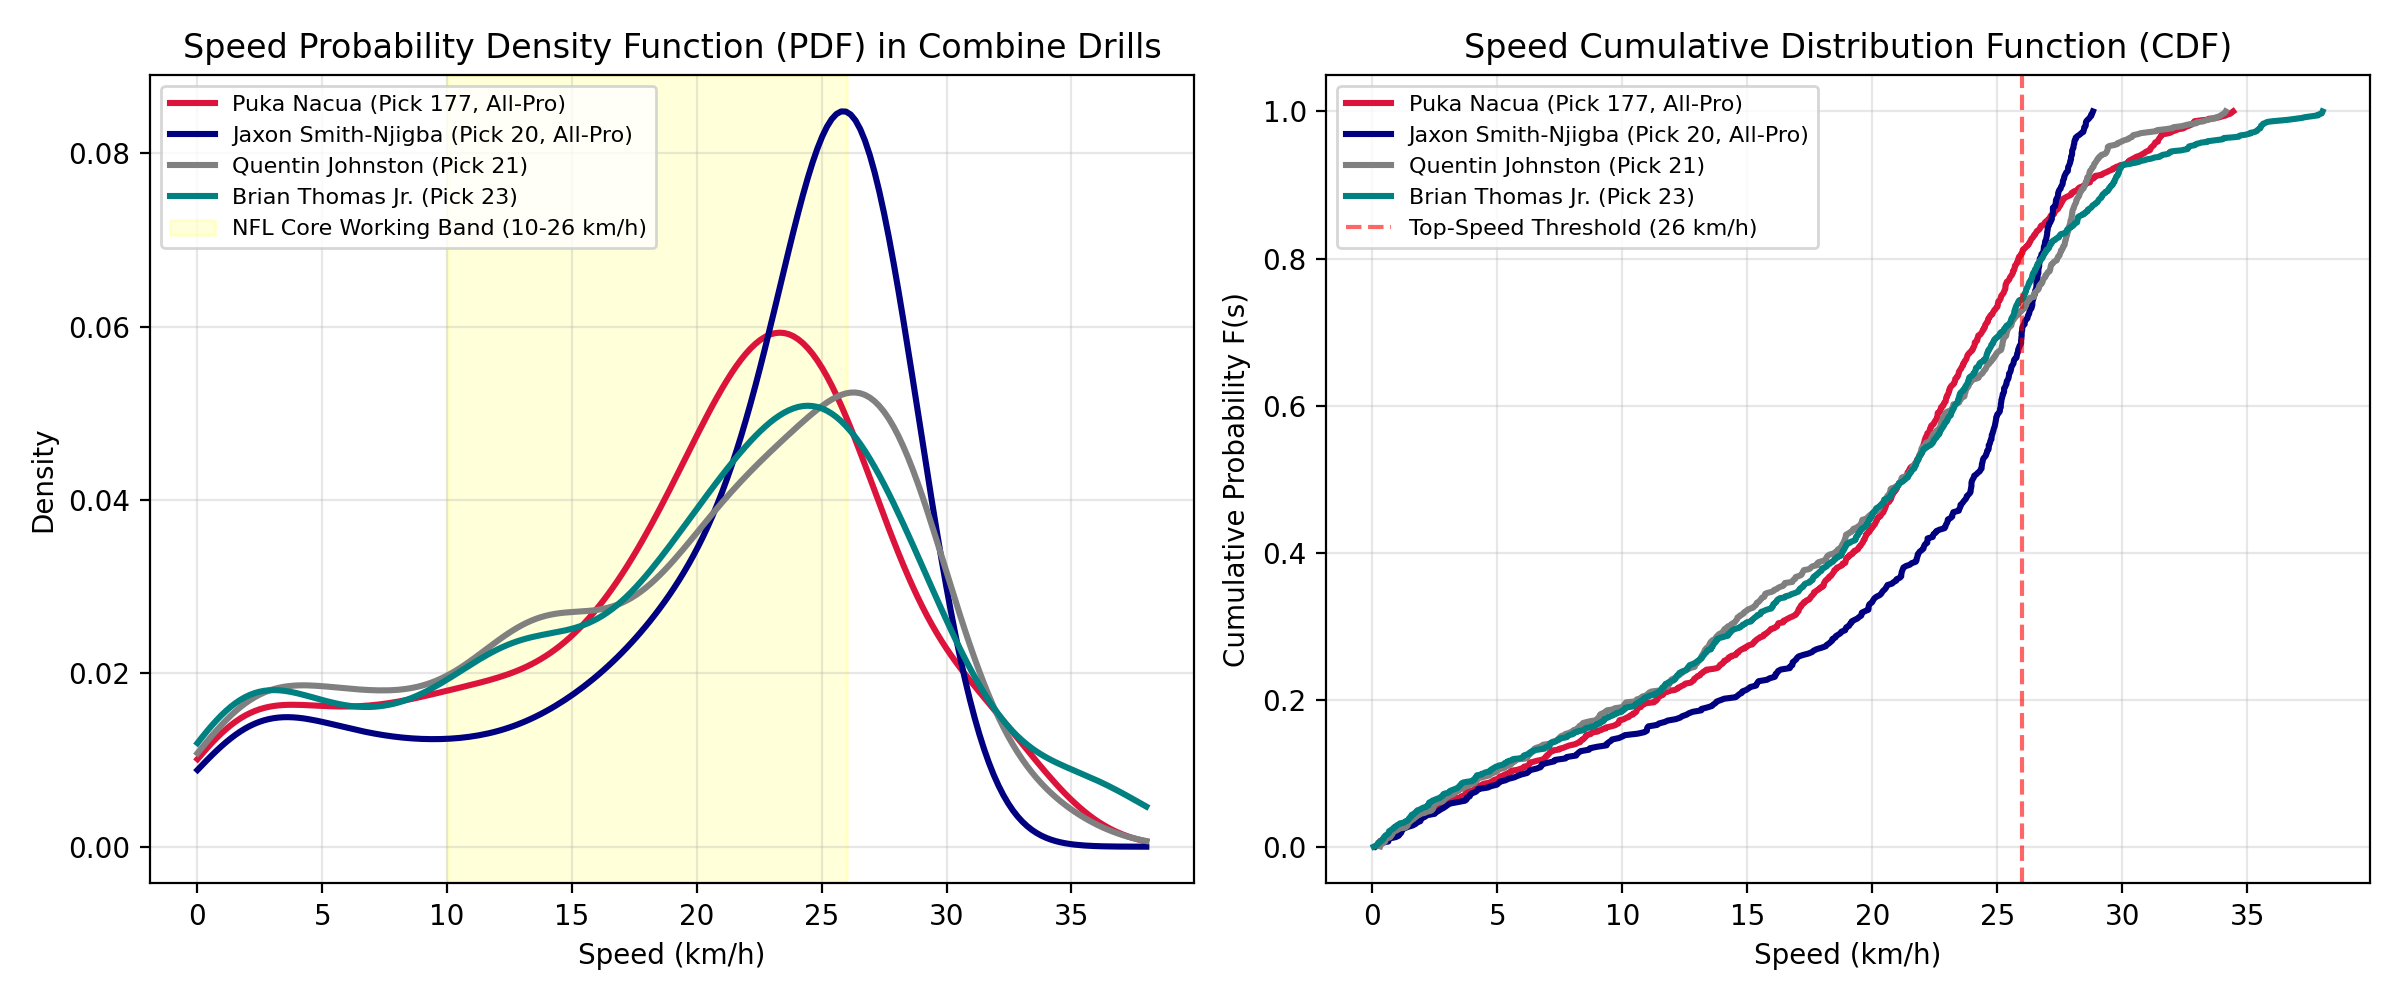
\includegraphics[keepaspectratio]{wr_speed_pdf_cdf.png}}

}

\caption{Figure 1: WR Speed PDF \& CDF Comparison}

\end{figure}%

\subsubsection{3.2 What the PDF and CDF
Reveal}\label{what-the-pdf-and-cdf-reveal}

In \textbf{Figure 1 (Left)}, Puka Nacua's density concentrates tightly
between \(20\text{ and }23\text{ km/h}\), with \(63.5\%\) of drill
frames in the Core Working Band. Brian Thomas Jr.~exhibits a long right
tail to \(38.0\text{ km/h}\)---an asset rarely engaged in standard route
trees.

In \textbf{Figure 1 (Right)}, Jaxon Smith-Njigba's CDF shifts furthest
right in the operating corridor: he never reached \(29\text{ km/h}\) at
the Combine, yet maintained the highest median cutting drill speed
(\(24.0\text{ km/h}\)). He generated separation by preserving velocity
through breaks rather than sprinting faster in a straight line.

\begin{center}\rule{0.5\linewidth}{0.5pt}\end{center}

\subsection{4. Biomechanical Analysis: Route Stem \& Break
Kinematics}\label{biomechanical-analysis-route-stem-break-kinematics}

To test whether high cut speed reflects elite technique or sloppy,
rounded routes, we analyze 10 Hz trajectories during the Comeback Route
drill (\texttt{COMEBACK\_ROUTE\_RIGHT}). The receiver drives an 18-yard
stem and cuts back at \(135^\circ\).

\begin{figure}[H]

{\centering \pandocbounded{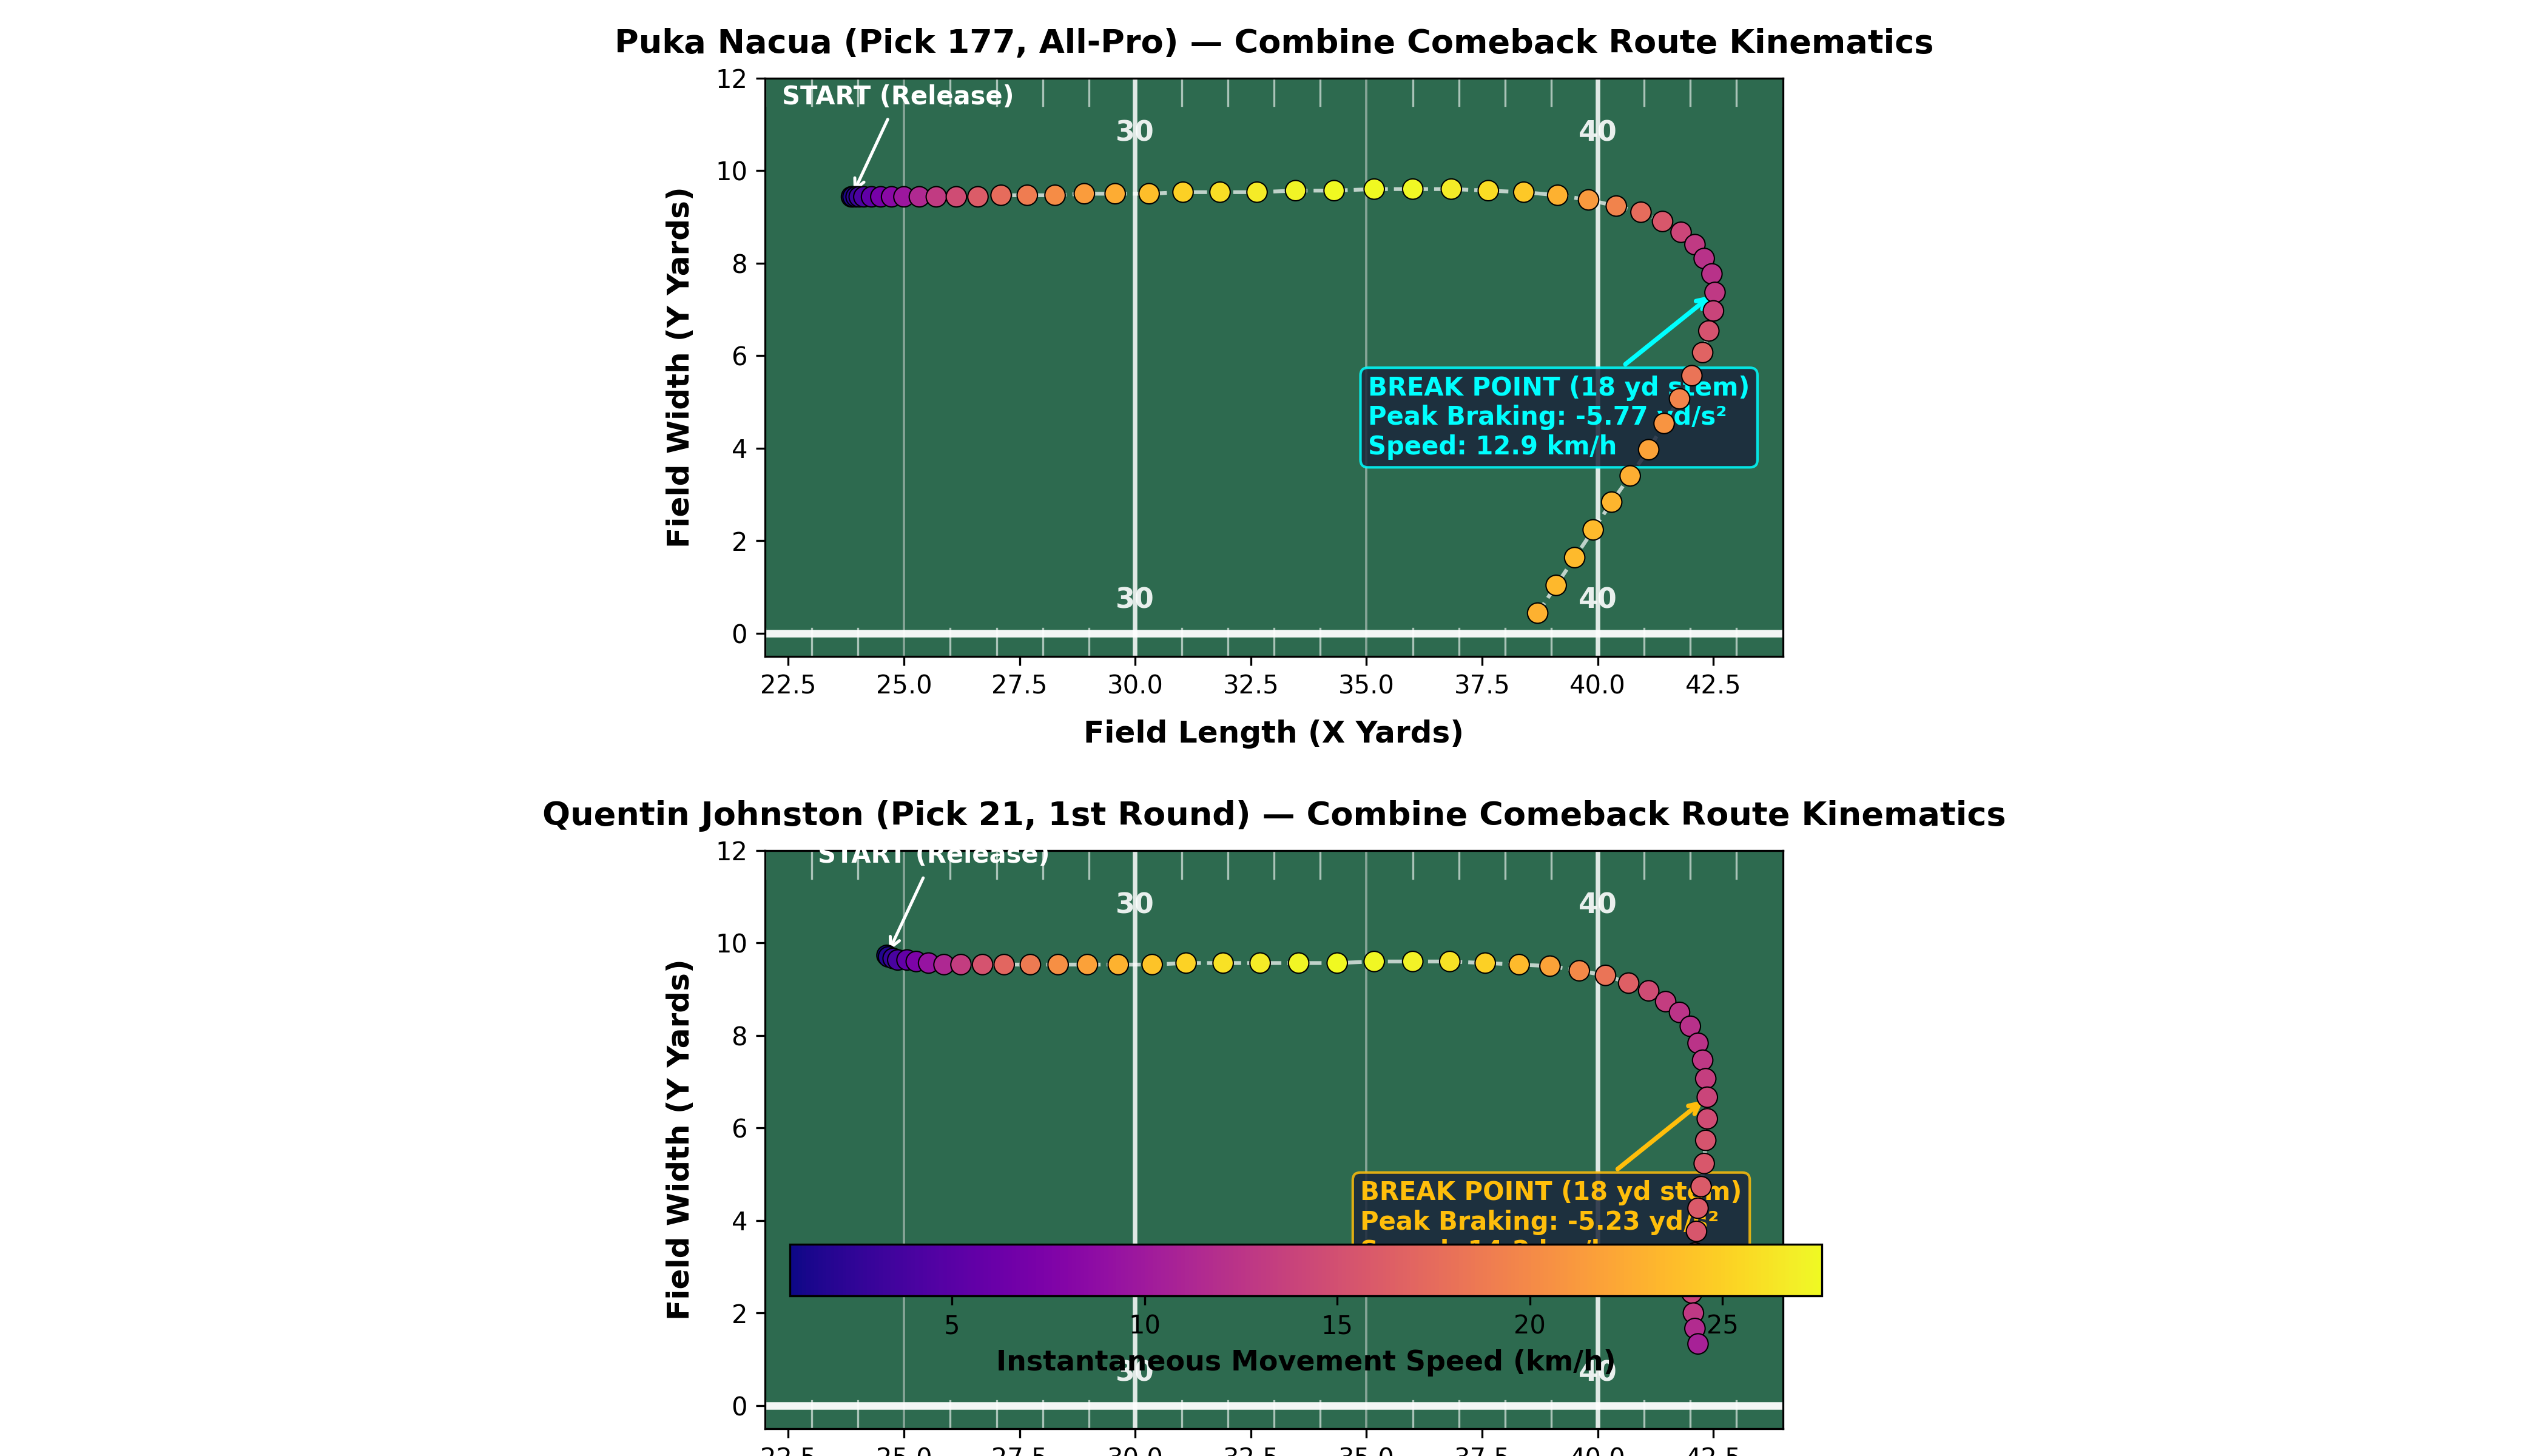
\includegraphics[keepaspectratio]{route_kinematics_field_plot.png}}

}

\caption{Figure 2: Regulation NFL Field Kinematics}

\end{figure}%

We compute trajectory curvature \(\kappa(t)\) and finite-difference
braking rate:
\[\kappa(t) = \frac{|\dot{x}\ddot{y} - \dot{y}\ddot{x}|}{(\dot{x}^2 + \dot{y}^2)^{3/2}}, \quad \text{Braking Rate} = \min_{t}\left(\frac{s(t) - s(t-\Delta t)}{\Delta t}\right)\]

In \textbf{Figure 2}: * \textbf{Puka Nacua:} Reaches break point at
\(X = 42.1\text{ yd}\) with peak braking of
\textbf{\(-5.77\text{ yd/s}^2\)}. He absorbs
\(708\text{ kg}\cdot\text{m/s}\) of momentum in \(0.8\text{ s}\) across
two strides, holding curvature at \(\kappa = 0.398\text{ m}^{-1}\) to
exit at \(17.8\text{ km/h}\). * \textbf{Quentin Johnston:} Displays peak
braking of \textbf{\(-5.23\text{ yd/s}^2\)}, requiring \(1.0\text{ s}\)
to decelerate. His path collapses into a sharp hitch
(\(\kappa = 0.973\text{ m}^{-1}\)), dropping exit speed to
\(12.4\text{ km/h}\).

Top performers do not round routes. They generate greater eccentric
braking impulse (\(\int \mathbf{F}_{\text{brake}}\,dt\)) to reverse
direction while conserving kinetic energy.

\begin{center}\rule{0.5\linewidth}{0.5pt}\end{center}

\subsection{5. Full Cohort Econometric
Models}\label{full-cohort-econometric-models}

We analyze all 106 Combine wide receivers participating in cutting
drills, partitioned into three empirical tiers: 1. \textbf{Top
Performers (\(N=16\)):} Multi-year starters (\(\ge 20\) starts), Pro
Bowlers, and All-Pros. 2. \textbf{Average Players (\(N=38\)):} Core
contributors (\(3\text{ to }19\) starts). 3. \textbf{Fringe Prospects
(\(N=52\)):} \(\le 2\) career starts.

{\def\LTcaptype{none} % do not increment counter
\begin{longtable}[]{@{}
  >{\raggedright\arraybackslash}p{(\linewidth - 8\tabcolsep) * \real{0.1667}}
  >{\centering\arraybackslash}p{(\linewidth - 8\tabcolsep) * \real{0.2083}}
  >{\centering\arraybackslash}p{(\linewidth - 8\tabcolsep) * \real{0.2083}}
  >{\centering\arraybackslash}p{(\linewidth - 8\tabcolsep) * \real{0.2083}}
  >{\centering\arraybackslash}p{(\linewidth - 8\tabcolsep) * \real{0.2083}}@{}}
\toprule\noalign{}
\begin{minipage}[b]{\linewidth}\raggedright
Performance Tier
\end{minipage} & \begin{minipage}[b]{\linewidth}\centering
N
\end{minipage} & \begin{minipage}[b]{\linewidth}\centering
Mean Cut Speed (\(s_{\text{cut}}\))
\end{minipage} & \begin{minipage}[b]{\linewidth}\centering
Std Dev (\(\sigma\))
\end{minipage} & \begin{minipage}[b]{\linewidth}\centering
Peak Sprint Speed
\end{minipage} \\
\midrule\noalign{}
\endhead
\bottomrule\noalign{}
\endlastfoot
\textbf{Top Performers} & 16 & \(17.84\text{ km/h}\) &
\(\pm 0.81\text{ km/h}\) & \(28.81\text{ km/h}\) \\
\textbf{Average Contributors} & 38 & \(17.04\text{ km/h}\) &
\(\pm 1.29\text{ km/h}\) & \(27.96\text{ km/h}\) \\
\textbf{Fringe Prospects} & 52 & \(16.30\text{ km/h}\) &
\(\pm 1.59\text{ km/h}\) & \(27.31\text{ km/h}\) \\
\end{longtable}
}

Welch's two-sample \(t\)-test confirms a large, significant difference
between Top and Fringe prospects (\(t = 3.723, p = 0.00041\), Cohen's
\(d = 1.08\)). Top receivers also exhibit half the standard deviation of
fringe players.

\subsubsection{5.1 Career Playing Time Model
(OLS)}\label{career-playing-time-model-ols}

We regress career offensive snaps on in-cut speed and 40-yard dash time:
\[\text{Snaps}_i = \beta_0 + \beta_1 (s_{\text{cut}, i}) + \beta_2 (\text{Forty}_i) + \epsilon_i\]

{\def\LTcaptype{none} % do not increment counter
\begin{longtable}[]{@{}
  >{\raggedright\arraybackslash}p{(\linewidth - 10\tabcolsep) * \real{0.1379}}
  >{\centering\arraybackslash}p{(\linewidth - 10\tabcolsep) * \real{0.1724}}
  >{\centering\arraybackslash}p{(\linewidth - 10\tabcolsep) * \real{0.1724}}
  >{\centering\arraybackslash}p{(\linewidth - 10\tabcolsep) * \real{0.1724}}
  >{\centering\arraybackslash}p{(\linewidth - 10\tabcolsep) * \real{0.1724}}
  >{\centering\arraybackslash}p{(\linewidth - 10\tabcolsep) * \real{0.1724}}@{}}
\toprule\noalign{}
\begin{minipage}[b]{\linewidth}\raggedright
Variable
\end{minipage} & \begin{minipage}[b]{\linewidth}\centering
Coefficient
\end{minipage} & \begin{minipage}[b]{\linewidth}\centering
Std. Error
\end{minipage} & \begin{minipage}[b]{\linewidth}\centering
\(t\)-statistic
\end{minipage} & \begin{minipage}[b]{\linewidth}\centering
\(p\)-value
\end{minipage} & \begin{minipage}[b]{\linewidth}\centering
95\% Conf. Interval
\end{minipage} \\
\midrule\noalign{}
\endhead
\bottomrule\noalign{}
\endlastfoot
\textbf{Intercept} & \(+1199.43\) & \(3120.64\) & \(+0.384\) & \(0.702\)
& \([-4997, +7396]\) \\
\textbf{In-Cut Speed (\(s_{\text{cut}}\))} & \(+132.09\) & \(42.27\) &
\(+3.125\) & \textbf{\(0.002\)} & \([+48.1, +216.0]\) \\
\textbf{40-Yard Dash} & \(-642.09\) & \(673.21\) & \(-0.954\) &
\(0.343\) & \([-1979, +695]\) \\
\end{longtable}
}

\emph{Dependent Variable: career\_offensive\_snaps \textbar{}
\(R^2 = 0.114\) \textbar{} \(N = 96\)}

Controlling for in-cut mechanics, the 40-yard dash is statistically
insignificant (\(p = 0.343\)). Each \(+1.0\text{ km/h}\) preserved
through cuts earns \(+132.1\) career snaps (\(p = 0.002\)).

\subsubsection{5.2 NFL Starter Probability
(Logit)}\label{nfl-starter-probability-logit}

We model the probability of becoming an established starter (\(\ge 10\)
starts):
\[\ln\left(\frac{P_i}{1 - P_i}\right) = \alpha + \beta_1 (s_{\text{cut}, i}) + \beta_2 (\text{Forty}_i)\]

{\def\LTcaptype{none} % do not increment counter
\begin{longtable}[]{@{}
  >{\raggedright\arraybackslash}p{(\linewidth - 10\tabcolsep) * \real{0.1379}}
  >{\centering\arraybackslash}p{(\linewidth - 10\tabcolsep) * \real{0.1724}}
  >{\centering\arraybackslash}p{(\linewidth - 10\tabcolsep) * \real{0.1724}}
  >{\centering\arraybackslash}p{(\linewidth - 10\tabcolsep) * \real{0.1724}}
  >{\centering\arraybackslash}p{(\linewidth - 10\tabcolsep) * \real{0.1724}}
  >{\centering\arraybackslash}p{(\linewidth - 10\tabcolsep) * \real{0.1724}}@{}}
\toprule\noalign{}
\begin{minipage}[b]{\linewidth}\raggedright
Variable
\end{minipage} & \begin{minipage}[b]{\linewidth}\centering
Coefficient
\end{minipage} & \begin{minipage}[b]{\linewidth}\centering
Std. Error
\end{minipage} & \begin{minipage}[b]{\linewidth}\centering
\(z\)-statistic
\end{minipage} & \begin{minipage}[b]{\linewidth}\centering
\(p\)-value
\end{minipage} & \begin{minipage}[b]{\linewidth}\centering
Odds Ratio
\end{minipage} \\
\midrule\noalign{}
\endhead
\bottomrule\noalign{}
\endlastfoot
\textbf{Intercept} & \(+16.544\) & \(13.765\) & \(+1.202\) & \(0.229\) &
--- \\
\textbf{In-Cut Speed (\(s_{\text{cut}}\))} & \(+0.569\) & \(0.221\) &
\(+2.575\) & \textbf{\(0.010\)} & \textbf{1.77×} \\
\textbf{40-Yard Dash} & \(-6.092\) & \(3.033\) & \(-2.009\) & \(0.045\)
& \(0.002×\) \\
\end{longtable}
}

\emph{Pseudo \(R^2 = 0.112\) \textbar{} LLR \(p = 0.0017\) \textbar{}
\(N = 96\)}

Each \(1.0\text{ km/h}\) increase in cut velocity preservation increases
starter odds by \(+77\%\)
(\(\text{OR} = 1.77, 95\%\text{ CI: } [1.15, 2.72]\)).

\begin{center}\rule{0.5\linewidth}{0.5pt}\end{center}

\subsection{\texorpdfstring{6. Trench Play \& Classical Mechanics:
Gamma-Over-Expected
(\(\gamma_{\text{OE}}\))}{6. Trench Play \& Classical Mechanics: Gamma-Over-Expected (\textbackslash gamma\_\{\textbackslash text\{OE\}\})}}\label{trench-play-classical-mechanics-gamma-over-expected-gamma_textoe}

In trench play, peak speed is irrelevant; downs are decided within
\(1.5\text{ s}\) via acceleration (\(\gamma\)). However, evaluating
acceleration directly violates Newton's Second Law
(\(\mathbf{F} = m\mathbf{a}\)). Because greater mass implies greater
inertia, peak acceleration decays with body weight.

We formulate \textbf{Gamma-Over-Expected (\(\gamma_{\text{OE}}\))} by
regressing 90th-percentile Combine acceleration (\(\gamma\)) on body
weight:
\[\mathbb{E}[\gamma_i \mid \text{Mass}_i] = \hat{\alpha} + \hat{\beta}(\text{Weight}_i), \quad \gamma_{\text{OE}, i} \equiv \gamma_{\text{observed}, i} - \mathbb{E}[\gamma_i \mid \text{Mass}_i]\]

\begin{figure}[H]

{\centering \pandocbounded{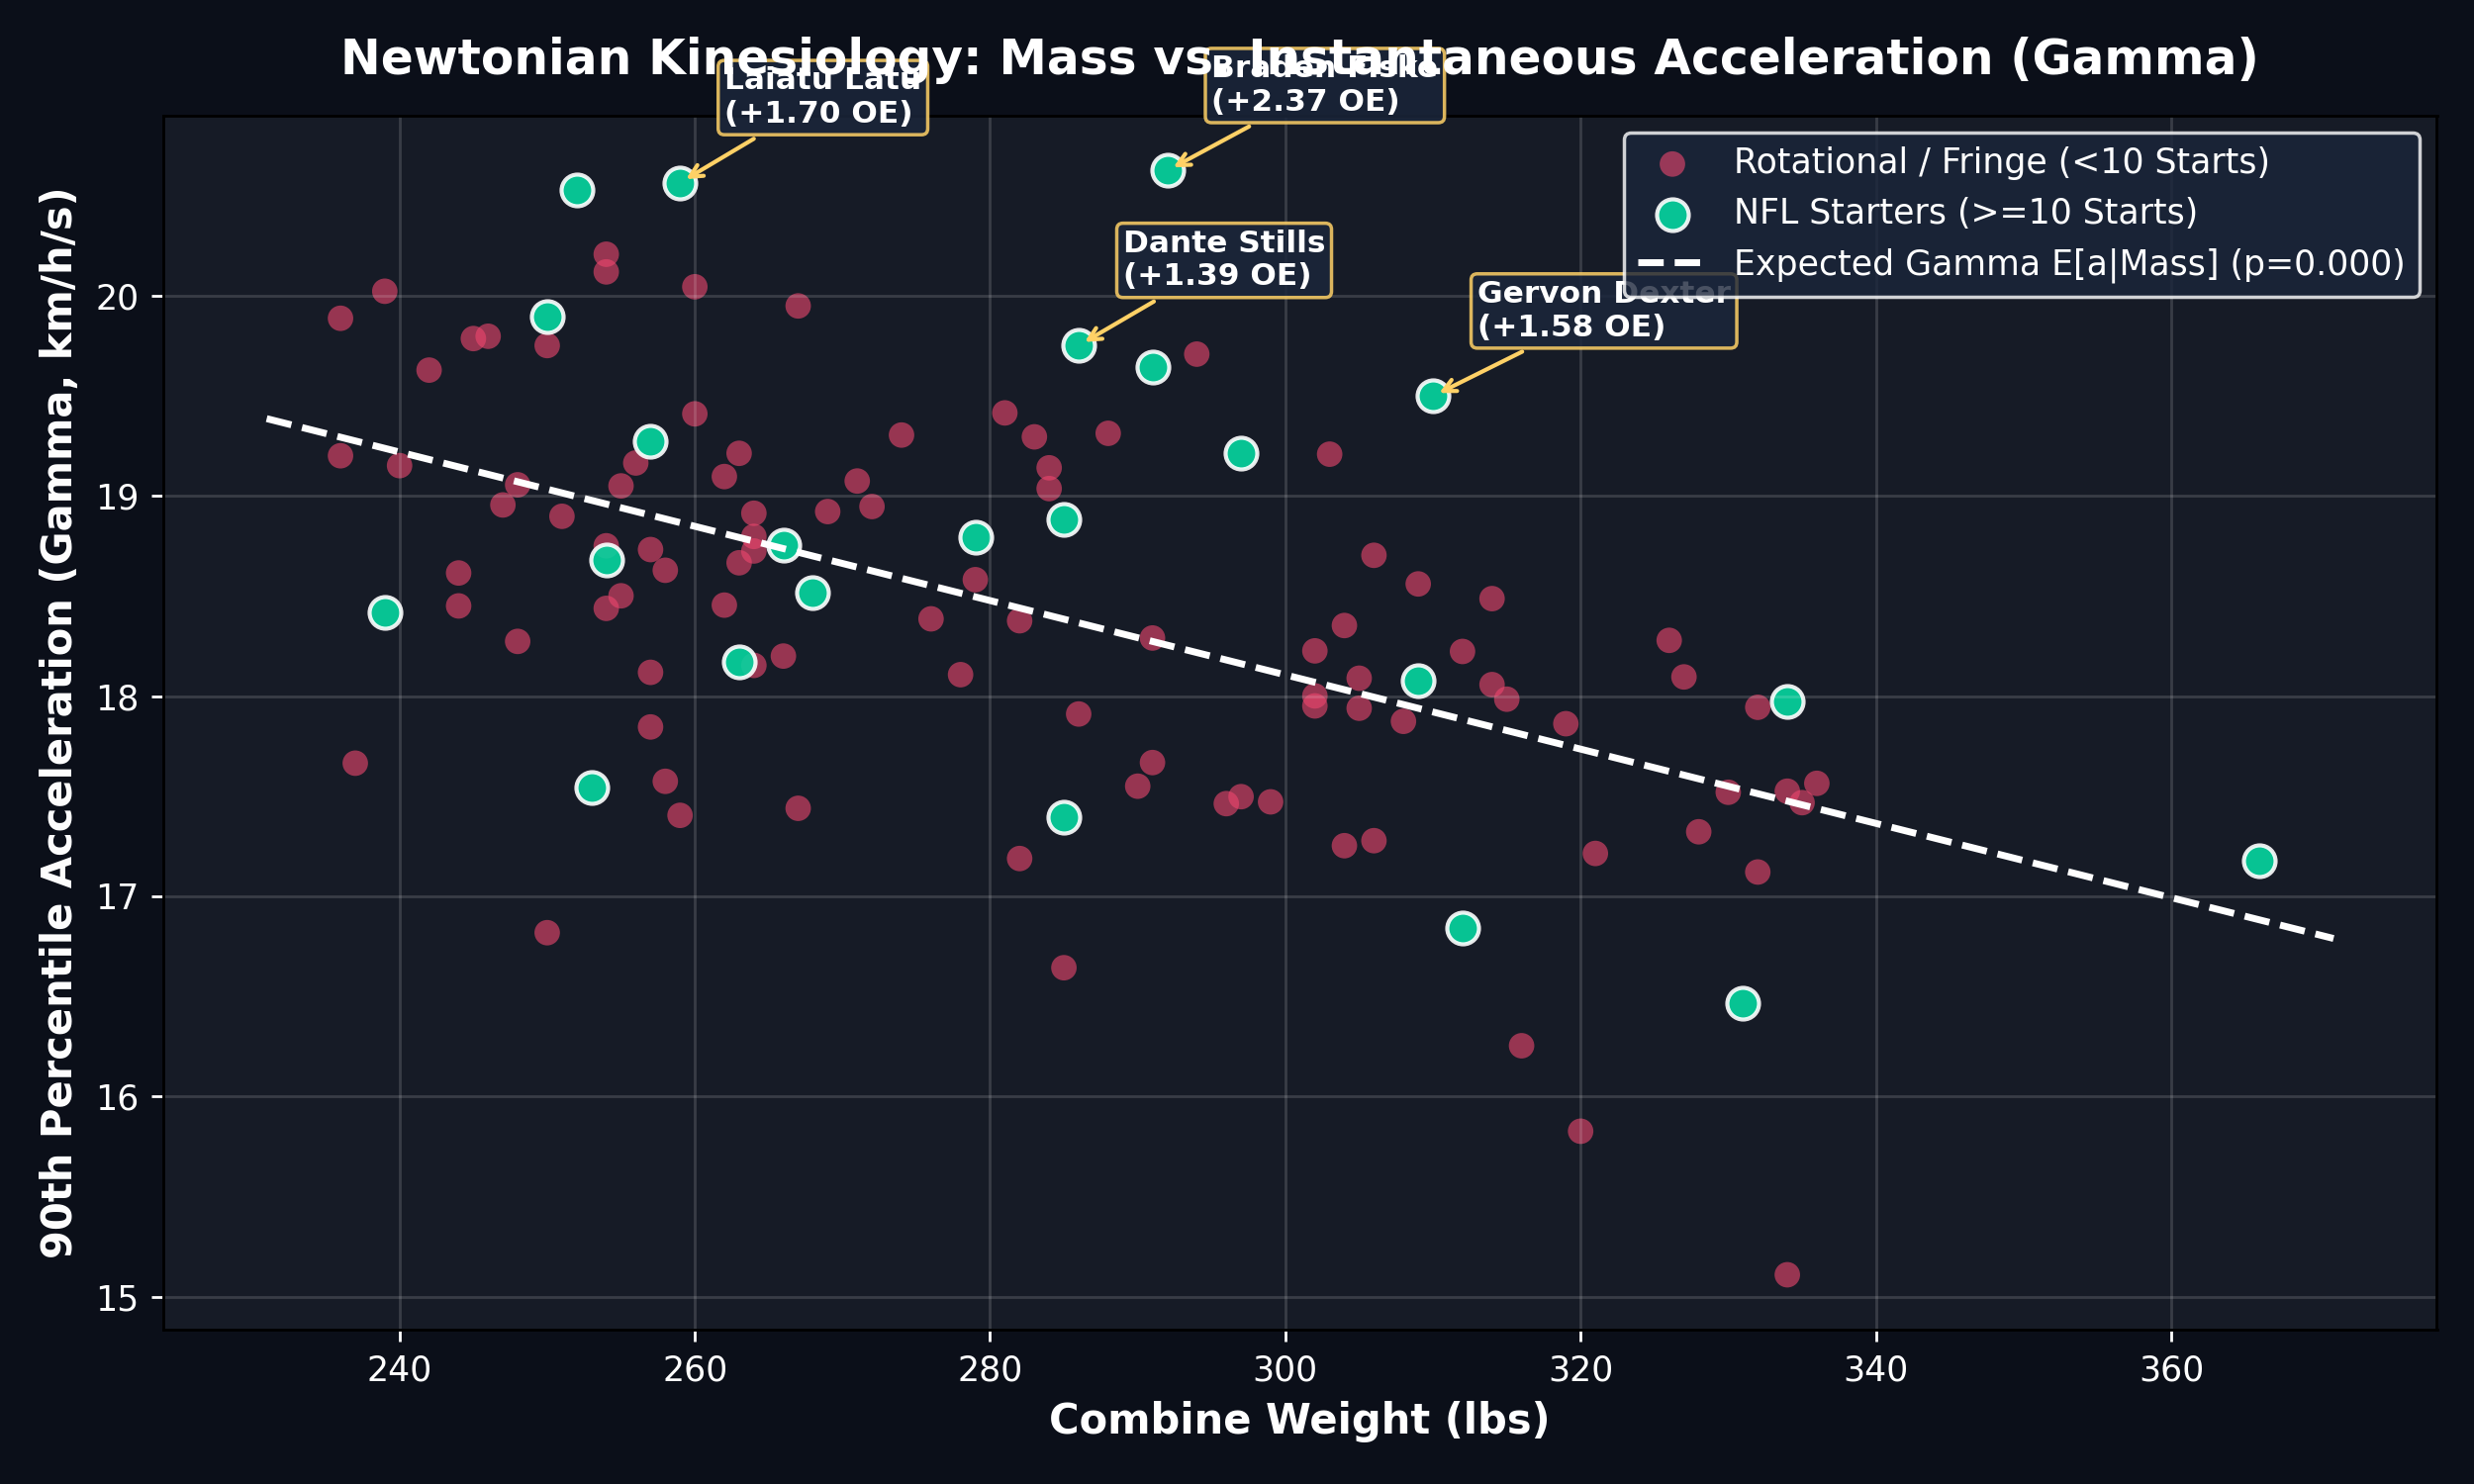
\includegraphics[keepaspectratio]{mass_vs_gamma_scatter.png}}

}

\caption{Figure 3: Mass vs.~Instantaneous Acceleration Scatter}

\end{figure}%

Modeling starter probability across 114 defensive linemen:
\[\ln\left(\frac{P_i}{1 - P_i}\right) = \beta_0 + \beta_1 (\gamma_{\text{OE}, i}) + \beta_2 (\text{Weight}_i)\]

{\def\LTcaptype{none} % do not increment counter
\begin{longtable}[]{@{}
  >{\raggedright\arraybackslash}p{(\linewidth - 10\tabcolsep) * \real{0.1379}}
  >{\centering\arraybackslash}p{(\linewidth - 10\tabcolsep) * \real{0.1724}}
  >{\centering\arraybackslash}p{(\linewidth - 10\tabcolsep) * \real{0.1724}}
  >{\centering\arraybackslash}p{(\linewidth - 10\tabcolsep) * \real{0.1724}}
  >{\centering\arraybackslash}p{(\linewidth - 10\tabcolsep) * \real{0.1724}}
  >{\centering\arraybackslash}p{(\linewidth - 10\tabcolsep) * \real{0.1724}}@{}}
\toprule\noalign{}
\begin{minipage}[b]{\linewidth}\raggedright
Variable
\end{minipage} & \begin{minipage}[b]{\linewidth}\centering
Coefficient
\end{minipage} & \begin{minipage}[b]{\linewidth}\centering
Std. Error
\end{minipage} & \begin{minipage}[b]{\linewidth}\centering
\(z\)-statistic
\end{minipage} & \begin{minipage}[b]{\linewidth}\centering
\(p\)-value
\end{minipage} & \begin{minipage}[b]{\linewidth}\centering
Odds Ratio
\end{minipage} \\
\midrule\noalign{}
\endhead
\bottomrule\noalign{}
\endlastfoot
\textbf{Intercept} & \(-2.652\) & \(2.315\) & \(-1.145\) & \(0.252\) &
--- \\
\textbf{Gamma-Over-Expected (\(\gamma_{\text{OE}}\))} & \(+0.615\) &
\(0.302\) & \(+2.035\) & \textbf{\(0.042\)} & \textbf{1.85×} \\
\textbf{Combine Weight} & \(+0.004\) & \(0.008\) & \(+0.504\) &
\(0.614\) & \(1.00×\) \\
\end{longtable}
}

Mass-adjusted acceleration is statistically significant
(\(p = 0.042, \text{OR} = 1.85\)). Each \(+1.0\text{ km/h/s}\) of
\(\gamma_{\text{OE}}\) increases starter odds by \(+85\%\), explaining
why Braden Fiske (\(292\text{ lbs}, \gamma_{\text{OE}} = +2.37\)) and
Laiatu Latu (\(259\text{ lbs}, \gamma_{\text{OE}} = +1.70\)) became
immediate multi-year starters.

\begin{center}\rule{0.5\linewidth}{0.5pt}\end{center}

\subsection{7. Actionable Draft Decision
Rules}\label{actionable-draft-decision-rules}

We summarize three decision rules for front offices:

{\def\LTcaptype{none} % do not increment counter
\begin{longtable}[]{@{}
  >{\raggedright\arraybackslash}p{(\linewidth - 6\tabcolsep) * \real{0.2500}}
  >{\raggedright\arraybackslash}p{(\linewidth - 6\tabcolsep) * \real{0.2500}}
  >{\raggedright\arraybackslash}p{(\linewidth - 6\tabcolsep) * \real{0.2500}}
  >{\raggedright\arraybackslash}p{(\linewidth - 6\tabcolsep) * \real{0.2500}}@{}}
\toprule\noalign{}
\begin{minipage}[b]{\linewidth}\raggedright
Position Group
\end{minipage} & \begin{minipage}[b]{\linewidth}\raggedright
Metric
\end{minipage} & \begin{minipage}[b]{\linewidth}\raggedright
Threshold
\end{minipage} & \begin{minipage}[b]{\linewidth}\raggedright
Front Office Decision
\end{minipage} \\
\midrule\noalign{}
\endhead
\bottomrule\noalign{}
\endlastfoot
\textbf{Wide Receivers} & In-Cut Speed (\(s_{\text{cut}}\)) &
\(s_{\text{cut}} \ge 17.0\text{ km/h}\) & Clear for Day 1/2 selection \\
\textbf{Wide Receivers} & In-Cut Speed (\(s_{\text{cut}}\)) &
\(s_{\text{cut}} < 16.0\text{ km/h}\) & Do not select on Days 1/2 \\
\textbf{Pass Rushers} & Gamma-Over-Expected (\(\gamma_{\text{OE}}\)) &
\(\gamma_{\text{OE}} \ge +1.50\text{ km/h/s}\) & Priority target (Day
2/3 value) \\
\textbf{Pass Rushers} & Gamma-Over-Expected (\(\gamma_{\text{OE}}\)) &
\(\gamma_{\text{OE}} < -1.00\text{ km/h/s}\) & Flag for low explosive
force \\
\textbf{All Prospects} & Core Band Occupancy &
\(\text{Occupancy} \ge 60\%\) & High regular-season translatability \\
\end{longtable}
}

\begin{enumerate}
\def\labelenumi{\arabic{enumi}.}
\tightlist
\item
  \textbf{The Workout Warrior Filter (WR):} If a receiver runs sub-4.40
  but records \(s_{\text{cut}} < 16.0\text{ km/h}\), do not draft on Day
  1 or Day 2. Their starter probability is \(<18\%\).
\item
  \textbf{The Trench Multiplier (DL/OL):} Target \(290+\text{ lb}\)
  linemen with \(\gamma_{\text{OE}} > +1.5\text{ km/h/s}\). Their
  mass-normalized force generates immediate pocket disruption regardless
  of baseline 40 time.
\item
  \textbf{Draft Density Over Tails:} Prioritize athletes whose speed
  density concentrates in the \(10\text{--}26\text{ km/h}\) Core Working
  Band over straight-line sprinters with unutilized high-speed tails.
\end{enumerate}

\begin{center}\rule{0.5\linewidth}{0.5pt}\end{center}

\subsection{8. Conclusion \& Open-Source
Deliverables}\label{conclusion-open-source-deliverables}

Continuous 10 Hz RFID tracking eliminates the epistemic limitations of
stopwatch scouting. Velocity preservation through cuts and mass-adjusted
explosive acceleration reliably differentiate NFL starters from fringe
prospects.

All analytical pipelines, interactive field viewers, and presentation
materials are available in the repository: * \textbf{Interactive Field
Tracking:}
\href{route_playback_interactive.html}{\texttt{route\_playback\_interactive.html}}
* \textbf{Cohort Density Viewer:}
\href{tier_comparison_pdf_cdf.html}{\texttt{tier\_comparison\_pdf\_cdf.html}}
* \textbf{LaTeX Beamer Deck:}
\href{presentation.pdf}{\texttt{presentation.pdf}} * \textbf{Formal
Research Paper:}
\href{report_assigned.pdf}{\texttt{report\_assigned.pdf}} *
\textbf{Replication Code:} Fully documented in \texttt{scripts/}.




\end{document}
